\hypertarget{SurrogateSplits_8c}{
\section{SurrogateSplits.c File Reference}
\label{SurrogateSplits_8c}\index{SurrogateSplits.c@{SurrogateSplits.c}}
}
{\tt \#include \char`\"{}party.h\char`\"{}}\par


Include dependency graph for SurrogateSplits.c:\nopagebreak
\begin{figure}[H]
\begin{center}
\leavevmode
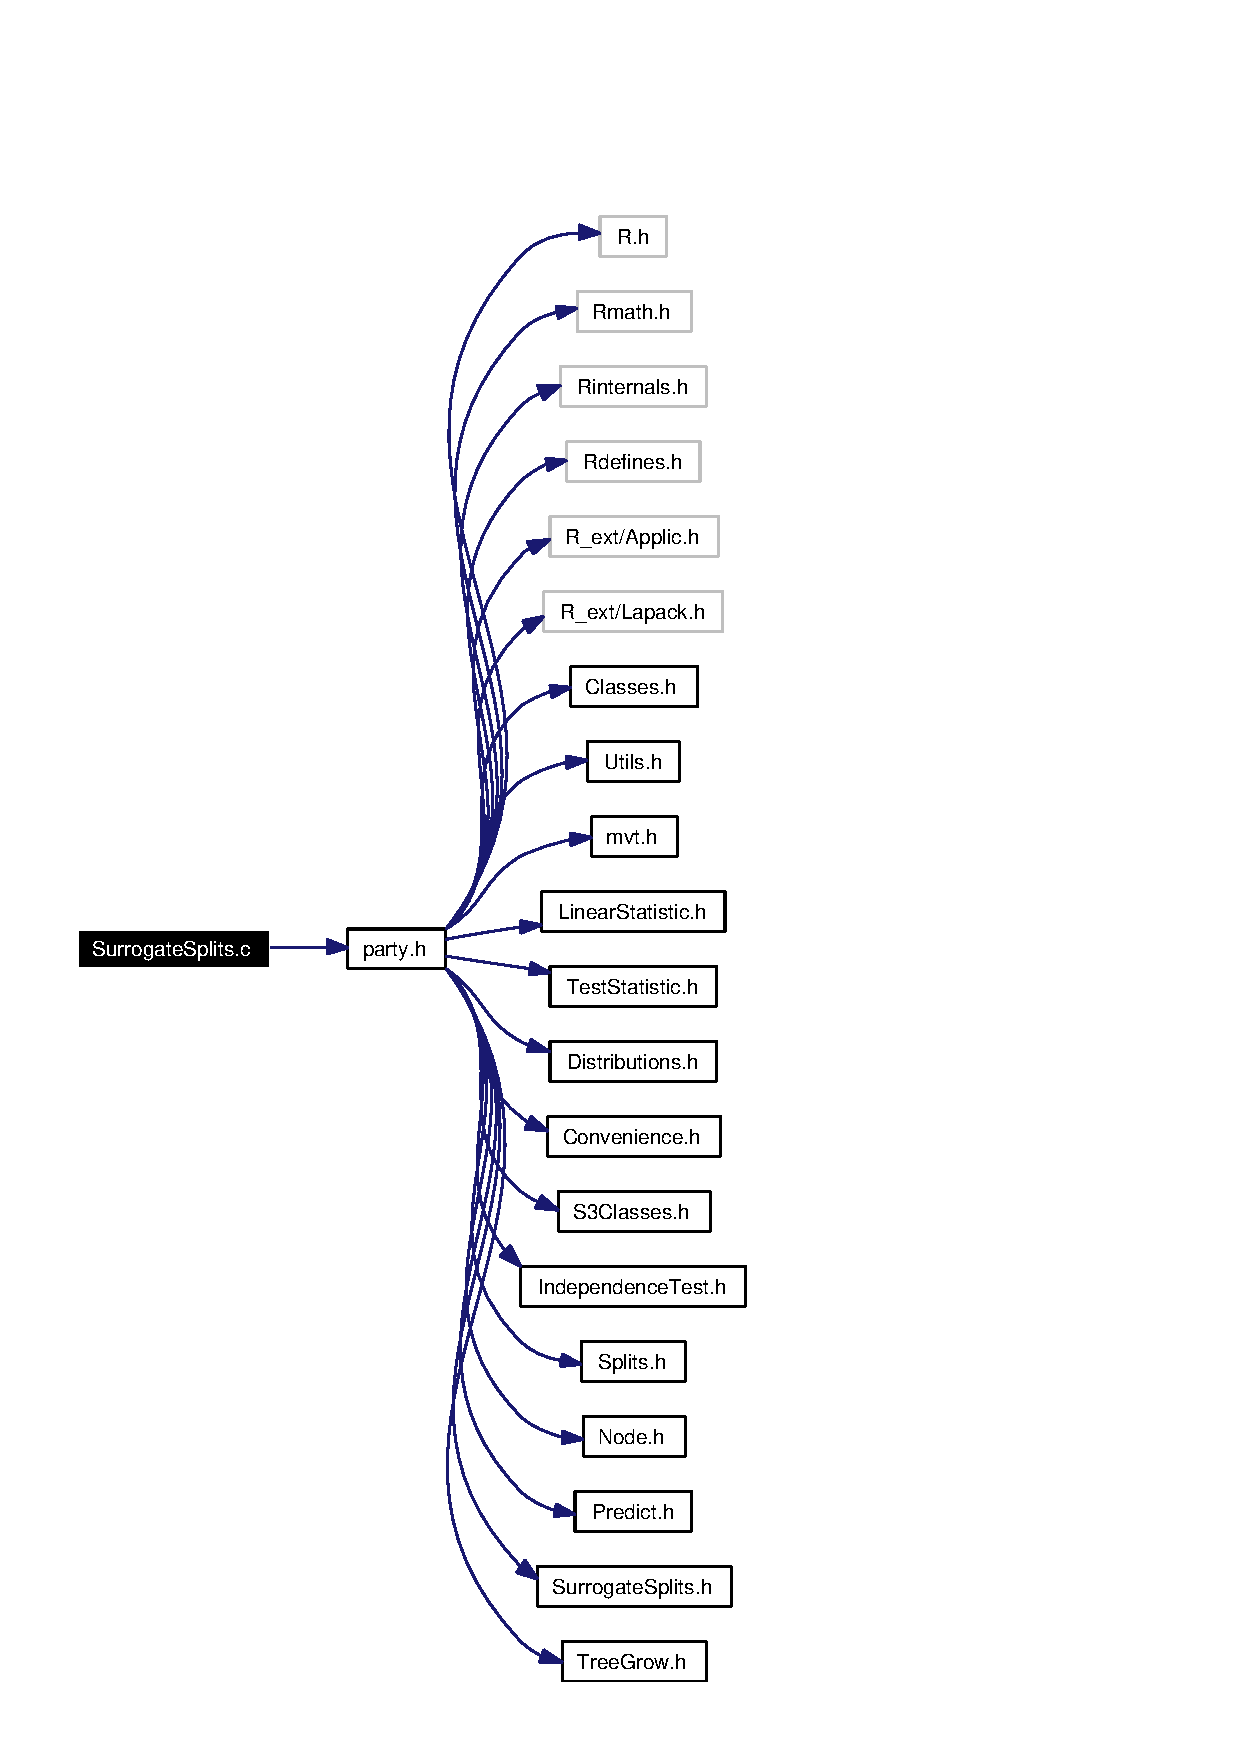
\includegraphics[width=420pt]{SurrogateSplits_8c__incl}
\end{center}
\end{figure}
\subsection*{Functions}
\begin{CompactItemize}
\item 
void \hyperlink{SurrogateSplits_8c_fd8931db67339ca2bb679d8d38135275}{C\_\-surrogates} (SEXP node, SEXP learnsample, SEXP weights, SEXP controls, SEXP fitmem)
\item 
SEXP \hyperlink{SurrogateSplits_8c_378f9c4110050c0d1762c6347d53379b}{R\_\-surrogates} (SEXP node, SEXP learnsample, SEXP weights, SEXP controls, SEXP fitmem)
\item 
void \hyperlink{SurrogateSplits_8c_6f9f8c3b4147854cacc43d67a055d911}{C\_\-splitsurrogate} (SEXP node, SEXP learnsample)
\end{CompactItemize}


\subsection{Detailed Description}
Suggorgate splits

\begin{Desc}
\item[Author:]\begin{Desc}
\item[Author]\end{Desc}
\end{Desc}
\begin{Desc}
\item[Date:]\begin{Desc}
\item[Date]\end{Desc}
\end{Desc}


Definition in file \hyperlink{SurrogateSplits_8c-source}{SurrogateSplits.c}.

\subsection{Function Documentation}
\hypertarget{SurrogateSplits_8c_6f9f8c3b4147854cacc43d67a055d911}{
\index{SurrogateSplits.c@{SurrogateSplits.c}!C_splitsurrogate@{C\_\-splitsurrogate}}
\index{C_splitsurrogate@{C\_\-splitsurrogate}!SurrogateSplits.c@{SurrogateSplits.c}}
\subsubsection{\setlength{\rightskip}{0pt plus 5cm}void C\_\-splitsurrogate (SEXP {\em node}, SEXP {\em learnsample})}}
\label{SurrogateSplits_8c_6f9f8c3b4147854cacc43d67a055d911}


Split with missing values \par
 \begin{Desc}
\item[Parameters:]
\begin{description}
\item[{\em node}]the current node with primary and surrogate splits specified \item[{\em learnsample}]learning sample \end{description}
\end{Desc}


Definition at line 173 of file SurrogateSplits.c.

Referenced by C\_\-TreeGrow().\hypertarget{SurrogateSplits_8c_fd8931db67339ca2bb679d8d38135275}{
\index{SurrogateSplits.c@{SurrogateSplits.c}!C_surrogates@{C\_\-surrogates}}
\index{C_surrogates@{C\_\-surrogates}!SurrogateSplits.c@{SurrogateSplits.c}}
\subsubsection{\setlength{\rightskip}{0pt plus 5cm}void C\_\-surrogates (SEXP {\em node}, SEXP {\em learnsample}, SEXP {\em weights}, SEXP {\em controls}, SEXP {\em fitmem})}}
\label{SurrogateSplits_8c_fd8931db67339ca2bb679d8d38135275}


Search for surrogate splits for bypassing the primary split \par
 \begin{Desc}
\item[Parameters:]
\begin{description}
\item[{\em node}]the current node with primary split specified \item[{\em learnsample}]learning sample \item[{\em weights}]the weights associated with the current node \item[{\em controls}]an object of class `TreeControl' \item[{\em fitmem}]an object of class `TreeFitMemory' \end{description}
\end{Desc}
\begin{Desc}
\item[\hyperlink{todo__todo000003}{Todo}]enable nominal surrogate split variables as well \end{Desc}


Definition at line 21 of file SurrogateSplits.c.

Referenced by C\_\-TreeGrow(), and R\_\-surrogates().\hypertarget{SurrogateSplits_8c_378f9c4110050c0d1762c6347d53379b}{
\index{SurrogateSplits.c@{SurrogateSplits.c}!R_surrogates@{R\_\-surrogates}}
\index{R_surrogates@{R\_\-surrogates}!SurrogateSplits.c@{SurrogateSplits.c}}
\subsubsection{\setlength{\rightskip}{0pt plus 5cm}SEXP R\_\-surrogates (SEXP {\em node}, SEXP {\em learnsample}, SEXP {\em weights}, SEXP {\em controls}, SEXP {\em fitmem})}}
\label{SurrogateSplits_8c_378f9c4110050c0d1762c6347d53379b}


R-interface to C\_\-surrogates \par
 \begin{Desc}
\item[Parameters:]
\begin{description}
\item[{\em node}]the current node with primary split specified \item[{\em learnsample}]learning sample \item[{\em weights}]the weights associated with the current node \item[{\em controls}]an object of class `TreeControl' \item[{\em fitmem}]an object of class `TreeFitMemory' \end{description}
\end{Desc}


Definition at line 158 of file SurrogateSplits.c.

References C\_\-surrogates(), and S3get\_\-surrogatesplits().

Here is the call graph for this function:\nopagebreak
\begin{figure}[H]
\begin{center}
\leavevmode
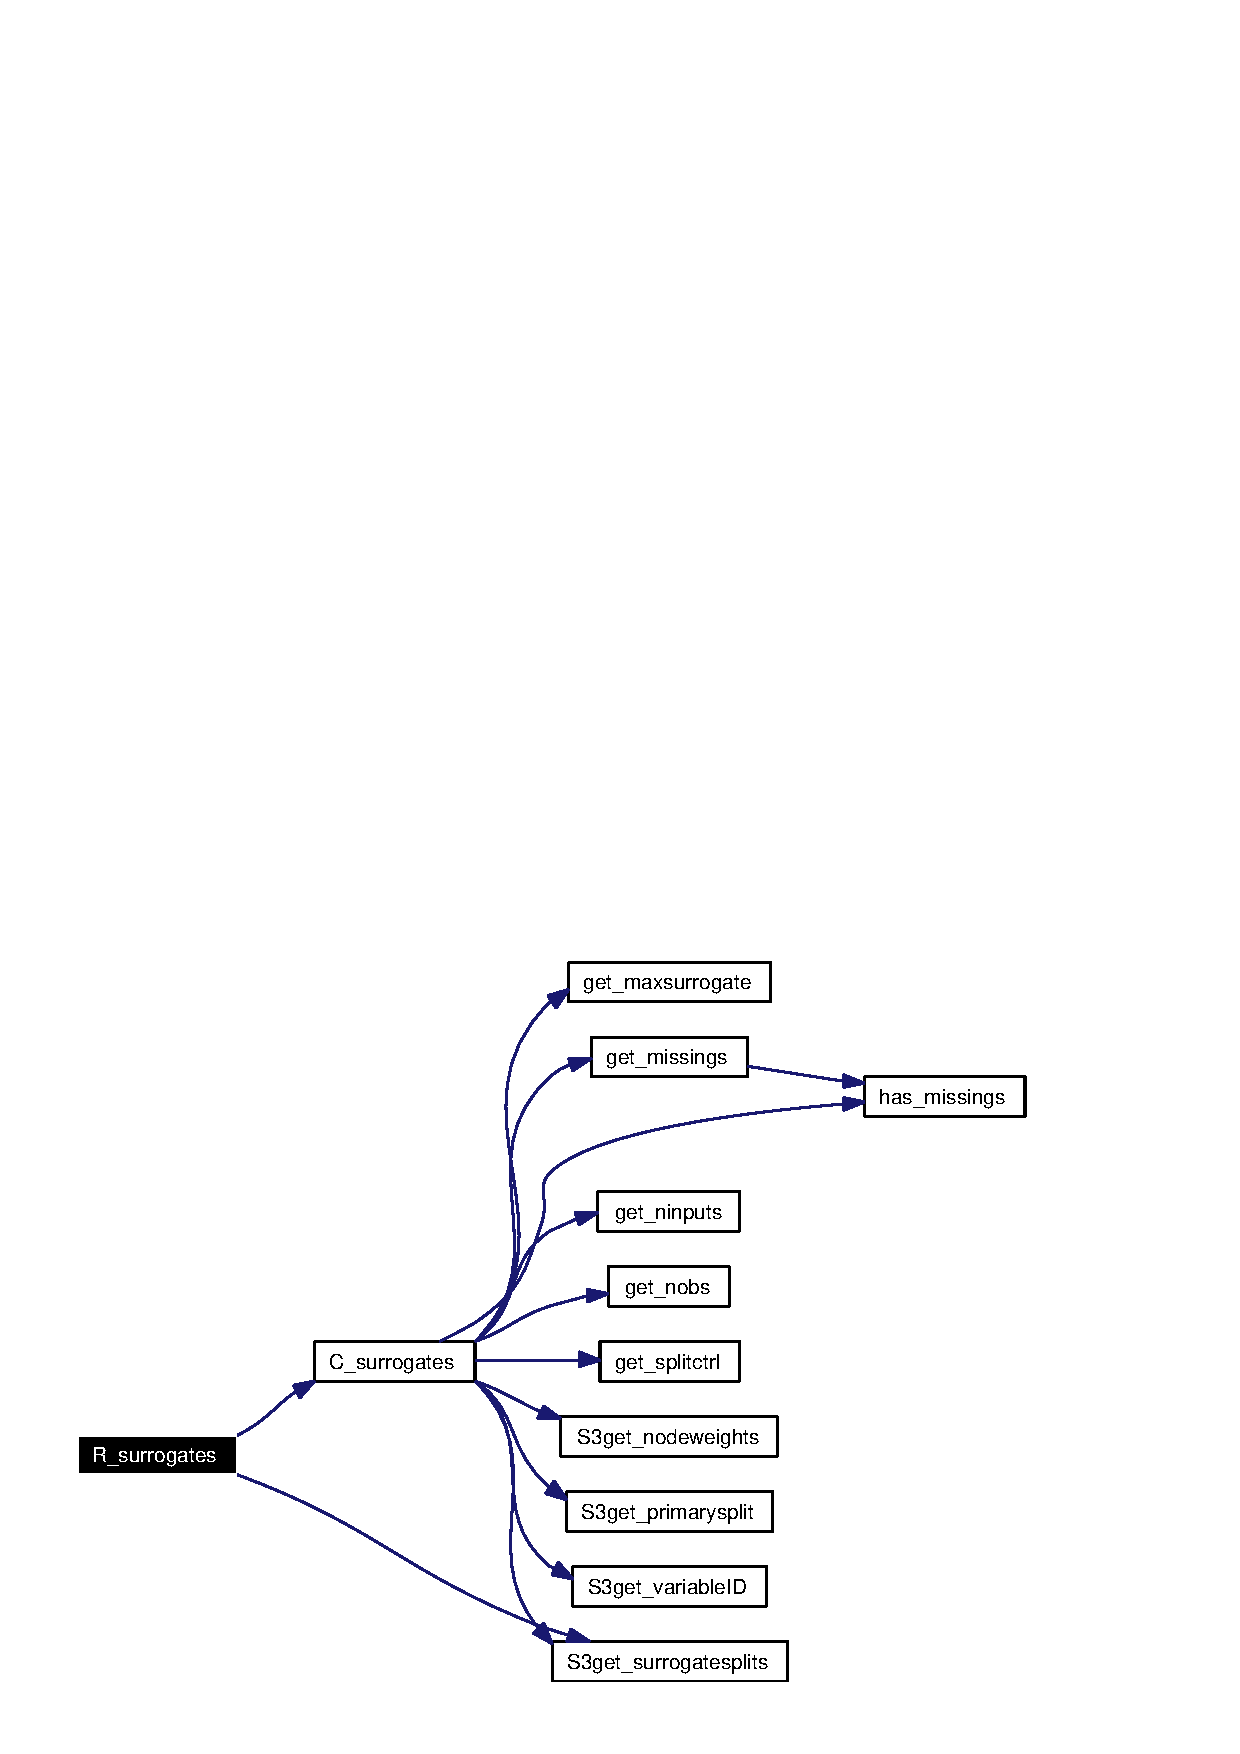
\includegraphics[width=141pt]{SurrogateSplits_8c_378f9c4110050c0d1762c6347d53379b_cgraph}
\end{center}
\end{figure}
